\subsubsection{Feature Distribution}\label{sec:impl-data-analysis:feature-dist}
Feature distribution is an integral part of an analysis, especially when some models utilized would be affected by it. It also provides further insight into the assumptions made about the data in question.

The purpose of the underlying section is to analyze the distribution of data for each feature present in the dataset. Additionally, it will be determined if any of the scaling methods applied have affected the data distribution.

\paragraph{Before Data Scaling}\label{sec:impl-data-analysis:feature-dist-before-scaling}
In order to determine the data distribution, the following methodology has been applied. 
To begin with, the mean and median was calculated for each feature to determine the skew of the data distribution. The skew has been determined by subtracting mean from median with negative values representing left skew and positive ones, a right skew to the distribution. The results of the operation can be observed in Figure \ref{fig:feature-dist:skew:unmodified-upsample}. It should be noted that for the unscaled data \fileAgeInSec{} feature has been removed as the result of $median - mean = -127705.55$ would completely overshadow the other metrics present in the graph. Suffice to say that \fileAgeInSec{} feature presented a significant left skewness of the data distribution in the unscaled dataset.

\begin{figure}[!h]
    \centering
    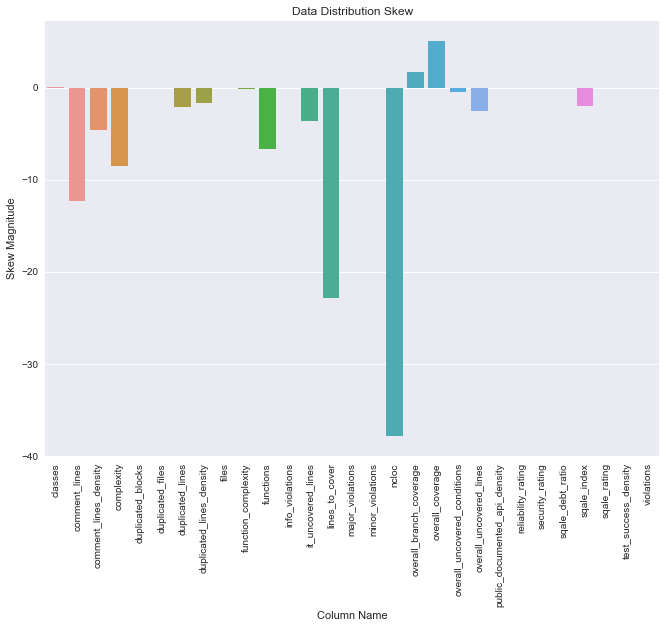
\includegraphics[scale=0.6]{Figures/feature-dist/Data_Distribution_Skew_unmodified_upsampled.png}
    \caption{Data distribution skew per feature: Up-sampled unscaled dataset}
    \label{fig:feature-dist:skew:unmodified-upsample}
\end{figure}

The actual feature distribution for unscaled up-sampled dataset can be viewed in Figure \ref{fig:feature-dist:upsampled-all-feature-dist}, where findings regarding skewness of the data, as depicted in Figure \ref{fig:feature-dist:skew:unmodified-upsample}, are confirmed.

\begin{figure}[!h]
    \centering
    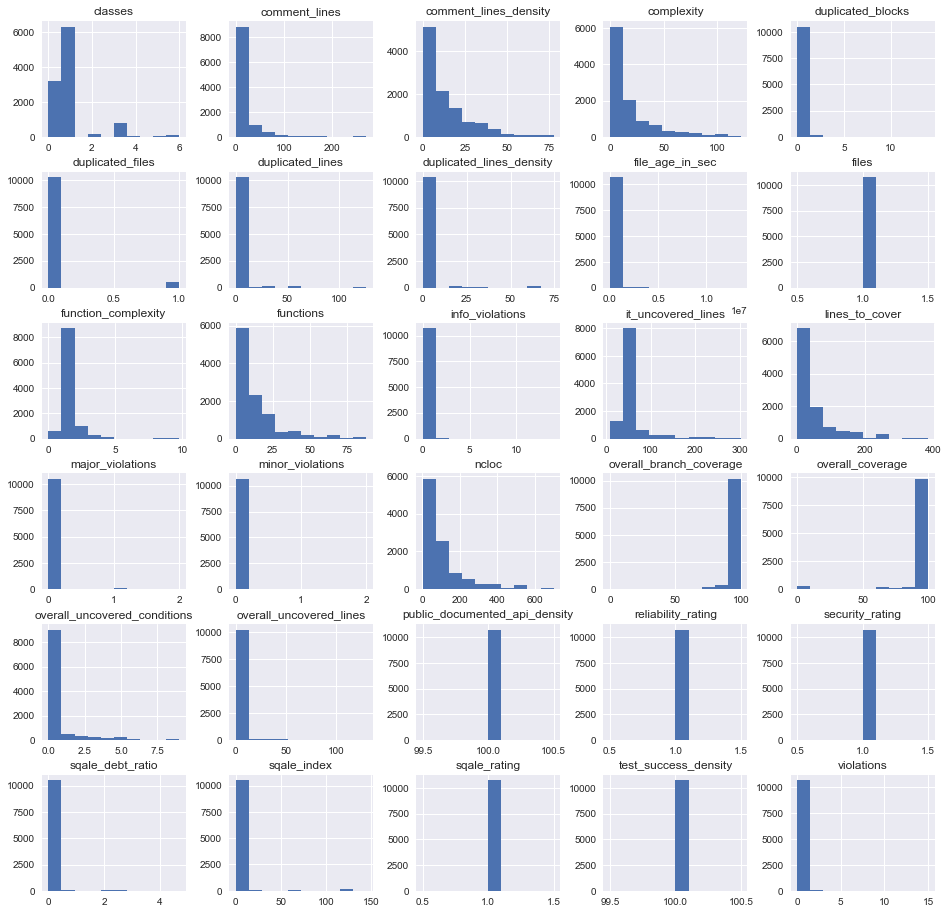
\includegraphics[scale=0.45]{Figures/feature-dist/attrib_dist_upscaled_unmod.png}
    \caption{Feature distribution: Up-sampled unscaled dataset}
    \label{fig:feature-dist:upsampled-all-feature-dist}
\end{figure}

Similar findings have been confirmed for the down-sampled dataset with Figure \ref{fig:feature-dist:downsampled-all-feature-dist} depicting the distribution per feature and Figure \ref{fig:feature-dist:skew:unmodified-upsample} showing the skewness of the data, as per previously listed calculation method.

\begin{figure}[!h]
    \centering
    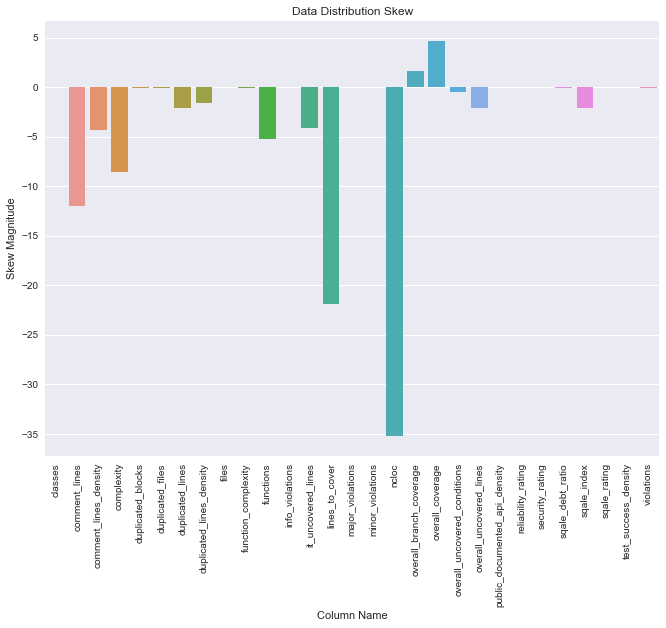
\includegraphics[scale=0.6]{Figures/feature-dist/Data_Distribution_Skew_unmodified_downsampled.png}
    \caption{Data distribution skew per feature: Down-sampled unscaled dataset}
    \label{fig:feature-dist:skew:unmodified-upsample}
\end{figure}

\begin{figure}[!h]
    \centering
    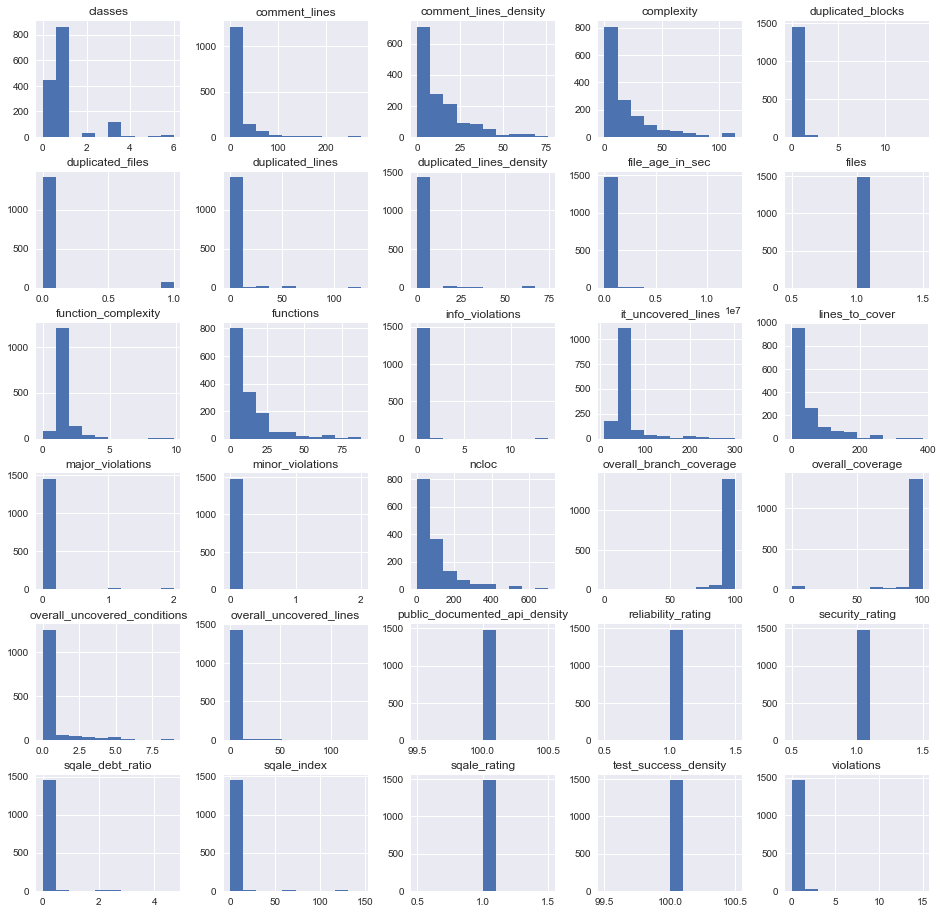
\includegraphics[scale=0.45]{Figures/feature-dist/attrib_dist_downscaled_unmod.png}
    \caption{Feature distribution: Down-sampled unscaled dataset}
    \label{fig:feature-dist:downsampled-all-feature-dist}
\end{figure}

Despite the data resampling process being random, it can be observed from the above figures that the data distribution and its skewness is approximately the same in both datasets. Therefore, it would stand to reason that the distribution after scaling has been applied to the dataset will exhibit the same pattern for both up-sampled and downsampled datasets.

\textbf{In conclusion}, most of the features in either resampled dataset exhibit a left skew in the data distribution. It is therefore assumed that any linear model analysis may be affected. It has been decided against redistributing the data at this stage as it is yet to be verified if data scaling will have any kind of an effect on the distribution of the feature data.
\FloatBarrier

\paragraph{After Data Scaling}\label{sec:impl-data-analysis:feature-dist-after-scaling}
Similarly to the process described in preceding Section \ref{sec:impl-data-analysis:feature-dist-before-scaling}, in order to determine the skewness of the data mean value has been subtracted from a median value per feature, per scaler applied. 

In comparison with the non-scaled datasets, whether upsampled or downsampled only small changes have been observed with regards to the magnitude of the data skew displayed in all features except \fileAgeInSec{}.
It has been observed that \fileAgeInSec{} feature has been scaled down significantly and as part of the process, the skew of the data observed in the unmodified datasets has been reduced significantly. 

The change in the data skew of \fileAgeInSec{} can be observed from Figures \ref{fig:} and \ref{fig:}

\begin{figure}
    \centering
    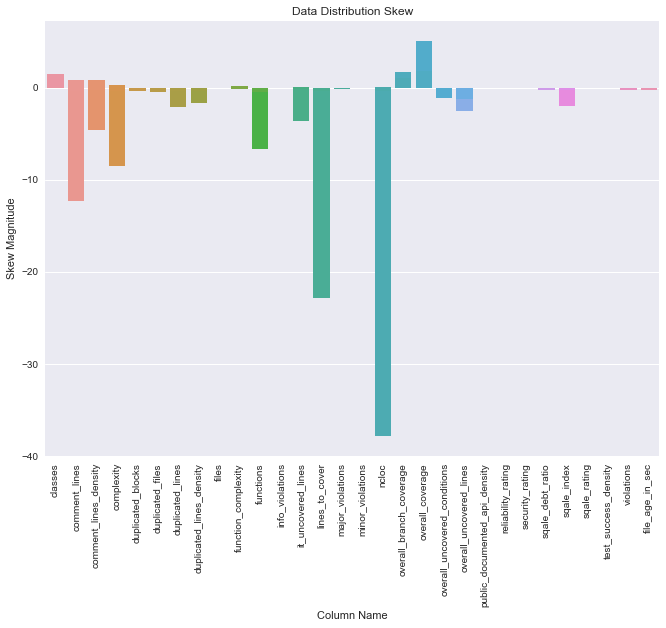
\includegraphics[scale=0.6]{Figures/feature-dist/Data_Distribution_Skew_quantile-normal_upsampled.png}
    \caption{Data distribution skew: Up-sampled dataset scaled with Quantile scaler - normal distribution}
    \label{fig:feature-dist:skew:quantile-normal-upsample}
\end{figure}

\begin{figure}
    \centering
    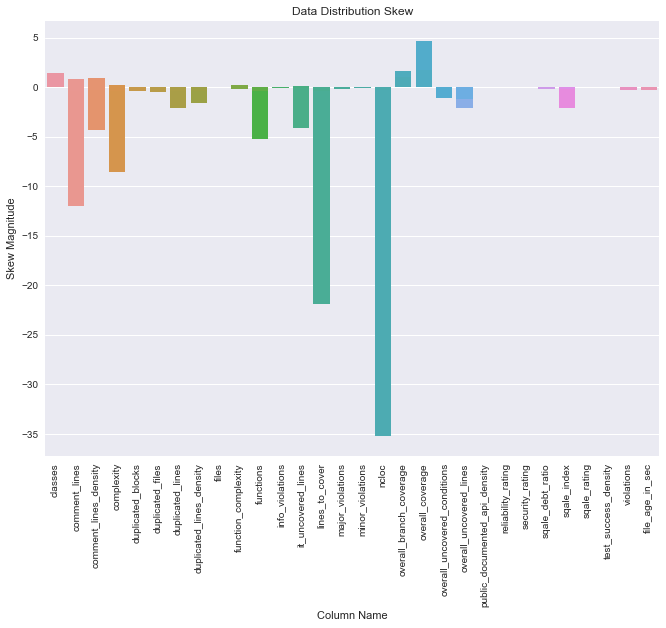
\includegraphics[scale=0.6]{Figures/feature-dist/Data_Distribution_Skew_quantile-normal_downsampled.png}
    \caption{Data distribution skew: Down-sampled dataset scaled with Quantile scaler - normal distribution}
    \label{fig:feature-dist:skew:quantile-normal-downsample}
\end{figure}

Additionally, after scalers have been applied a small difference in the skewness of the data has been observed between up and down-sampled datasets. In general, upsampled datasets had more features exhibiting 0 skewness factor, metric calculated as per formula listed in Section \ref{sec:impl-data-analysis:feature-dist-before-scaling}. Furthermore, the skewness factor for features that failed to achieve the 0 score have been slightly larger in the up-sampled dataset. 
However, given that the differences observed in data distribution after that scaling operation has been carried out were not significant, bar the expected change in \fileAgeInSec{}, it has been decided to carry on with the analysis as is.

\textbf{In conclusion} only in the case of one feature, the \fileAgeInSec{}, the scaling operations have had any significant impact on the distribution of the data and its skewness. Other features, exhibited minute changes that should not affect the underlying analysis.
\FloatBarrier